\chapter{Stratified flow in a channel (Viollet)}

\section{Purpose}

This test demonstrates the ability of \telemac{3D} to model thermal and stratified flow.

\section{Description}

The test case considers the stable configuration of Pierre-Louis Viollet’s experimentation
(1980) with a Froude number of 0.9, which consists in a 2 layer flow of same height,
$h$ = 0.1~m.
The lower layer has a velocity $U_2$ and a temperature $T_2$.
The upper layer has a velocity $U_1 < U_2$ and a temperature $T_1 > T_2$.

The configuration is a rectangular channel with length = 10~m (100$h$)
and width = 1~m (10$h$).
The bottom has a regular slope with a channel tilt = 5.30921 $\times$ 10$^{-6}$,
see Figure \ref{fig:Viollet:Bottom}.

\begin{figure}[H]
 \centering
 \includegraphicsmaybe{[width=\textwidth]}{../img/Bottom.png}
  \caption{Bottom elevation.}\label{fig:Viollet:Bottom}
\end{figure}

\subsection{Initial and Boundary Conditions}

The computation is initialised with a constant heigth equal to 0.2~m (2$h$),
horizontal velocity along $x$ = $U_1$ = $U_2$ = 0.05~m/s
and $T_1$ = 25.35~$^\circ$C for the upper fluid and $T_2$ = 20~$^\circ$C
for the lower fluid.

The boundary conditions are:
\begin{itemize}
\item For the solid walls, a slip condition on channel banks is used for the
velocities,
\item On the bottom, a Haaland law with coefficient equal to 63.4505112
is prescribed,
\item Upstream a flowrate equal to 0.01~m$^3$/s is prescribed,
\item Downstream the water level is equal to 0.19995~m.
\end{itemize}

A double logarithmic velocity profile is imposed for the lower layer and
a logarithmic profile for the upper layer
(see Figure \ref{fig:Viollet:ExpConfig}) according
the following formulae defined in the \telfile{USER\_BORD3D} subroutine:

\begin{equation}
  u(z_1) = \frac{u_1^*}{\kappa}\left( \log \left( \frac{z_1}{\xi_s}\right) + 8.5 \right)
\end{equation}

\begin{equation}
  u(z_2) = \frac{u_2^*}{\kappa}\left( \log \left( \frac{\min(z_2, h-z_2)}{\xi_s}\right) + 8.5 \right)
\end{equation}

\begin{equation}
  u(z=0) = u(z=h) = \frac{u_2^*}{\kappa}\left( \log \left( \frac{0.1 \times dz}{\xi_s}\right) + 8.5 \right)
\end{equation}

where $z_1$ and $z_2$ are the levels in upper and lower layers
respectively (starting from the lower level of each layer).
$\xi_s$ = 10$^{-4}$~m et $dz$ is the distance between two planes
(i.e. $dz = h/26$ since there are 27 planes).

Upstream $k$ and $\epsilon$ profiles are imposed according the following
formulae defined in the \telfile{KEPCL3} subroutine:

\begin{equation}
  k(z_1) = n_{turb} u_{z=h}^{2} \left( 1-\frac{z_1}{h}\right)
\end{equation}

\begin{equation}
  \epsilon(z_1) = \frac{C_\mu^{3/4}}{\kappa} \frac{k_{z=0}^{3/2}}{\max(z_1, \delta)}
\end{equation}

\begin{equation}
  k(z_2) = n_{turb} u_{z=0}^{2}
\end{equation}

\begin{equation}
  \epsilon(z_2) = \frac{C_\mu^{3/4}}{\kappa} \frac{k_{z=0}^{3/2}}{\max(\min(z_2,h-z_2), \delta)}
\end{equation}

where $n_{turb}$ = 5 $\times$ 10$^{-3}$, $C_\mu$ = 0.09 and
$\delta = 10^{-6}$.

Surface and bottom boundary condition for $\epsilon$ are defined in the
\telfile{KEPICL} subroutine: Neumann at bottom and Dirichlet at surface.

\begin{figure}[H]
 \centering
 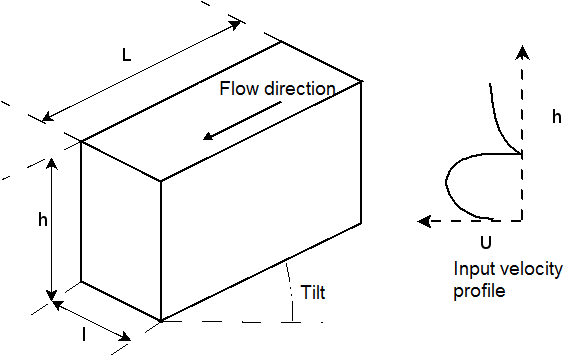
\includegraphics[width=0.9\textwidth]{./img/exp_config.png}
 \caption{Physical configuration of the experiment.}
 \label{fig:Viollet:ExpConfig}
\end{figure}

\subsection{Mesh and numerical parameters}

The 2D mesh (Figure \ref{fig:Viollet:Mesh}) is made of 1,280 triangular elements
(697 nodes).

27 planes are regularly spaced on the vertical ($\sigma$ transformation,
see Figure \ref{fig:Viollet:MeshV}).

\begin{figure}[H]
 \centering
 \includegraphicsmaybe{[width=\textwidth]}{../img/Mesh.png}
  \caption{Horizontal mesh.}\label{fig:Viollet:Mesh}
\end{figure}

\begin{figure}[H]
 \centering
 \includegraphicsmaybe{[width=\textwidth]}{../img/MeshV.png}
  \caption{Vertical mesh.}\label{fig:Viollet:MeshV}
\end{figure}

The time step is 0.1~s for a simulated period of 500~s (8~min 20~s).

The non-hydrostatic version is used.

To solve the advection, the N-type MURD (scheme 4) is used for the velocities,
temperature and $k$-$\epsilon$.

The default solvers (GMRES for propagation and PPE, conjugate gradient for
diffusion of velocities, tracers and $k$-$\epsilon$) are used.
For every solving operation, asked accuracy is quite fine
(from 10$^{-16}$ for temperature and $k$-$\epsilon$ to 10$^{-16}$ for PPE and
propagation steps).

\subsection{Physical parameters}

The $k$-$\epsilon$ model is used for turbulence modelling in both vertical and
horizontal directions
(\telkey{VERTICAL TURBULENCE MODEL = HORIZONTAL TURBULENCE MODEL = 3})
with \telkey{PRANDTL NUMBER} = 0.71 and \telkey{KARMAN CONSTANT} = 0.41.

\telkey{COEFFICIENT FOR VERTICAL DIFFUSION OF TRACERS} is set to
1.44.10$^{-7}$~m$^2$/s.

Density law is a function of temperature (\telkey{DENSITY LAW} = 1).

\subsection{Comments}

It should be noted that a bias exists in the measures presented:
the channel inlet flow does not correspond to the integral of the
measured speeds on the section.
This comes probably from measurement error of the velocity field.
The velocity been the field that is sought to be reproduced, the
measured velocity field is corrected by multiplying it by a constant.
No correction is applied to temperature measurements.

\section{Results}

Figure \ref{fig:Viollet:velo_temp_profiles} presents velocity and temperature
profiles comparisons at $x/h$ = 10, 30 and 100 between \telemac{3D} results and
corrected experimental measurement of P.-L. Viollet, for the stable
stratification case with $Fr$ = 0.9.
The comparisons show a good match between simulation results and
measurements.
The evolution of the velocity and temperature profiles at the different
sections of the channel is well reproduced.

\begin{figure}[H]
\centering
\begin{minipage}[t]{.45\textwidth}
 \centering
\includegraphicsmaybe{[width=\textwidth]}{../img/velocity_profile_10.png}
\end{minipage}
\begin{minipage}[t]{.45\textwidth}
 \centering
\includegraphicsmaybe{[width=\textwidth]}{../img/temp_profile_10.png}
\end{minipage}
\begin{minipage}[t]{.45\textwidth}
 \centering
\includegraphicsmaybe{[width=\textwidth]}{../img/velocity_profile_30.png}
\end{minipage}
\begin{minipage}[t]{.45\textwidth}
 \centering
\includegraphicsmaybe{[width=\textwidth]}{../img/temp_profile_30.png}
\end{minipage}
\begin{minipage}[t]{.45\textwidth}
 \centering
\includegraphicsmaybe{[width=\textwidth]}{../img/velocity_profile_100.png}
\end{minipage}
\begin{minipage}[t]{.45\textwidth}
 \centering
\includegraphicsmaybe{[width=\textwidth]}{../img/temp_profile_100.png}
\end{minipage}
 \caption{Velocity and temperature profiles comparisons at $x/h$ = 10, 30 and 100 between \telemac{3D} and corrected experimental measurement of P.-L. Viollet, for the stable stratification case with $Fr$ = 0.9.}
 \label{fig:Viollet:velo_temp_profiles}
\end{figure}

\section{Conclusion}

\telemac{3D} is capable to model thermal and stratified flow.
